
%%%%%%%%%%%%%%%%%%%%%%%%%%%%----->SECCIÓN 4<-----%%%%%%%%%%%%%%%%%%%%%%%%%
\newpage

\chapter{Influencia de la atmósfera en el flujo de secundarios}

\noindent Una vez construidos y validados los perfiles atmosféricos, es hora de analizar el efecto que éstos tienen en el flujo de secundarios, para ello, se realizan simulaciones de flujo con las condiciones iniciales establecidas en la sección 2.1. En total, son 12 simulaciones usando un perfil atmosférico mensual a la vez, y finalmente una última simulación, usando el perfil atmosférico predeterminado subtropical. El resultado, se observa en la figura \ref{fig:fig19}.\\

\begin{figure}[htb!]
\centering
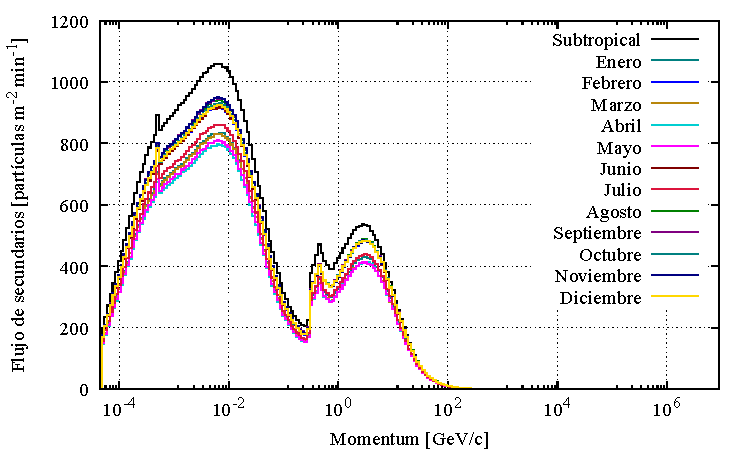
\includegraphics[width=1\textwidth]{Figs/flux_bucaramanga_1212.pdf}
\caption[Flujo de secundarios en función de la energía a la altura de Bucaramanga.]{Simulación del flujo total de secundarios en función de la energía a la altura de Bucaramanga, usando diferentes medios de interacción: La línea negra corresponde al perfil predeterminado subtropical, y las líneas de colores, corresponde a los 12 perfiles atmosféricos mensuales. Las estimaciones arrojan un flujo mayor con el perfil subtropical, en comparación a los 12 perfiles atmosféricos mensuales, siendo la mayor diferencia observada con el mes de abril.}
\label{fig:fig19}
\end{figure}
Las estimaciones arrojan un flujo mayor con el perfil subtropical, en comparación a los 12 perfiles atmosféricos mensuales, siendo la mayor diferencia observada con el mes de abril. La primera prominencia corresponde a la contribución al flujo, de la componente electromagnética, y la segunda está compuesta de dos picos que corresponden al aporte de los neutrones y muones respectivamente.\\ 

La figura \ref{fig:fig20} muestra el espectro de secundarios, que permite ver de forma más clara, la componentes del flujo, diferenciado por el tipo de partículas que lo componen. Ha sido obtenido usando el perfil atmosférico del mes de abril. Aquí, se puede apreciar que el aporte de los neutrones al segundo pico es significativo sólo entre los $0.2$ a $1 GeV/c$ y disminuye drásticamente a medida que aumenta en energía. A diferencia de la componente muónica que incrementa en ese mismo rango de energía, teniendo su máximo valor cerca a los $10 GeV/c$.\\
\begin{figure}[htb!]
\centering
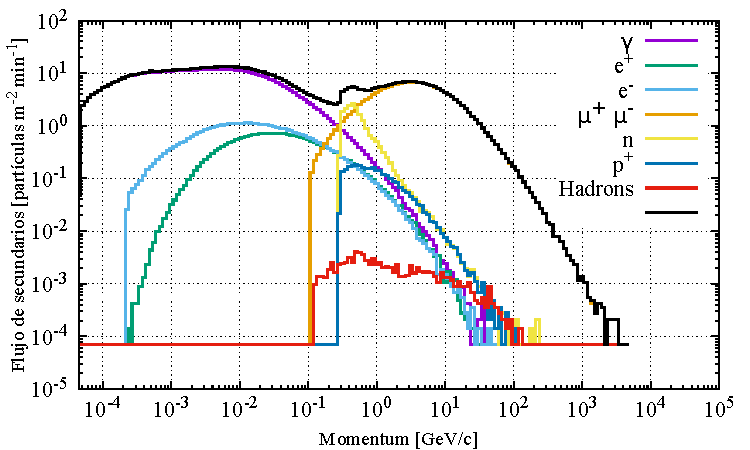
\includegraphics[width=1\textwidth]{Figs/flux_bucaramanga_ALL_PARTICLES_1212.pdf}
\caption[Espectro de energía de secundarios a la altura de Bucaramanga]{Simulación del espectro de energía de secundarios a la altura de Bucaramanga, usando el perfil atmosférico para el mes de abril, como medio de interacción. En negro se representa el espectro total de secundarios, en morado la contribución de los fotones, en celeste los electrones, en verde los positrones, en naranja los muones y antimuones, en amarillo los neutrones, en azul oscuro los protones y en rojo los hadrones.}
\label{fig:fig20}
\end{figure}\\
%10,219358835
%9,582708804 con el mes de noviembre
%, que para un tiempo de 4 horas, con el perfil atmosférico Subtropical es esperaban 3.319$x10^{6}$ muones, y con el perfil atmosférico de abril, se obtendrían 7.4$x10^{5}$ menos.
De la simulación representada en la figura \ref{fig:fig19}, se obtiene una diferencia en el flujo total entre 10,22$\%$ y el 24,12$\%$ correspondientes a los meses de noviembre y abril respectivamente. De forma similar, para los muones estas diferencias están entre 9,58$\%$ y 22,25$\%$. Este resultado responde finalmente a la interrogante planteada en el capítulo anterior. Además, permite concluir que las variaciones atmosféricas a lo largo del año, pueden ser evidenciadas en el flujo de secundarios a nivel del suelo, incluso en regiones tropicales como Bucaramanga.\\

Sin embargo, aún se debe comprobar que las diferencias en el flujo de secundarios observadas, obedezcan a la modulación que inducen las variaciones de temperatura a lo largo del año. La figura \ref{fig:fig21} muestra el cambio mensual del flujo obtenido con los nuevos perfiles atmosféricos creados para el año 2018, en comparación al flujo que se obtiene con el perfil atmosférico subtropical, que es constante a lo largo del año. Se observan diferencias significativas, siendo mayores en el primer semestre. Una explicación a este comportamiento está relacionado con los cambios de clima, y puede apreciarse en el diagrama de la derecha.\\

\begin{figure}[htb!]
\centering
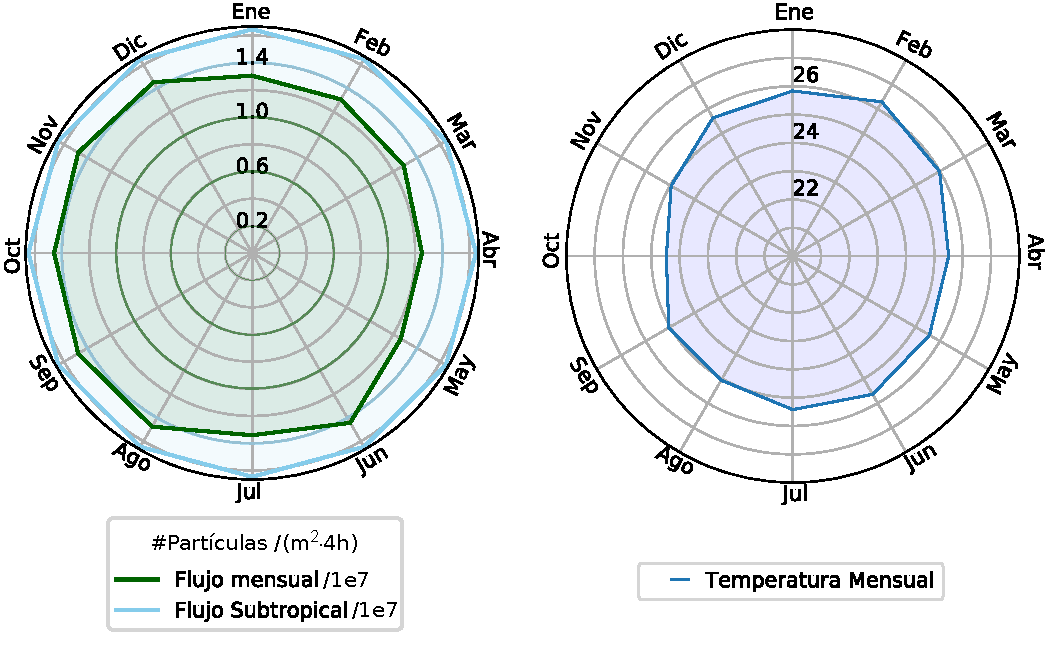
\includegraphics[width=0.8\textwidth]{Figs/Flujo_TEMP.pdf}
\caption[Comparación del flujo, atmósferas mensuales vs perfil predeterminado.]{A la derecha diagrama que compara el cambio mensual del flujo obtenido a partir de los perfiles atmosféricos construidos para el año 2018, y el flujo que se obtiene con el perfil atmosférico subtropical, que es constante a lo largo del año. Se observan diferencias significativas, siendo mayores en el primer semestre del año. A la izquierda temperatura promedio para cada mes del año 2018 para la ciudad de Bucaramanga. Se observa un aumento de la temperatura en el primer semestre del año, que contrasta con la disminución en el flujo para ese mismo intervalo de tiempo. Los datos de temperatura están disponibles en la base de datos de RACIMO AIRE. \citep{Datos}}
\label{fig:fig21}
\end{figure}

Se observa una relación inversa entre el flujo y los cambios de temperatura, en concordancia con la aproximación de gas ideal, es decir, a medida que la temperatura aumenta, disminuye la densidad, por ende, también disminuye el flujo de secundarios. Este resultado, es una evidencia de que los perfiles atmosféricos construidos no sólo reproducen bien el comportamiento de la atmósfera a lo largo del año, sino que permiten incluso observar en el flujo de secundarios, las variaciones de temperatura. \\

Como comprobación final, se hicieron simulaciones de la distribución longitudinal de secundarios, esta vez observando el efecto que tiene cambiar el perfil atmosférico, en una EAS generada por diferentes tipos de primarios como veremos a continuación.\\

\textbf{Efecto de los perfiles atmosféricos en EAS generadas por partículas individuales:} Para estudiar el comportamiento de los perfiles atmosféricos mensuales durante el desarrollo de la lluvia, se realizan simulaciones de partículas individuales. Para tener suficientes datos estadísticos, se realizan  10 simulaciones de EAS para primarios de $1\cdot 10^{8}$ GeV, 1000 para primarios de $1\cdot 10^{6}$ GeV, y 5000 para $1\cdot 10^{3}$ GeV.\\

Con el resultado de estas simulaciones, se realizan promedios estadísticos que permiten obtener la distribución longitudinal más cercana de lo que se pudiera observar en la realidad.  La figura \ref{fig:fig23} muestra el resultado de promediar la distribución longitudinal de un protón de $1\cdot 10^{6} GeV$ que fue simulado 1000 veces, observando el número de partículas  generado, a medida que éstas se propagan por la atmósfera (A),  la diferencia porcentual usando el perfil atmosférico predeterminado y para el mes de enero (B), la energía depositada a lo largo de dicha dirección de propagación (C) y la diferencia porcentual entre la energía depositada en los dos medios de propagación (D).\\

\begin{figure}[htb!]
\centering
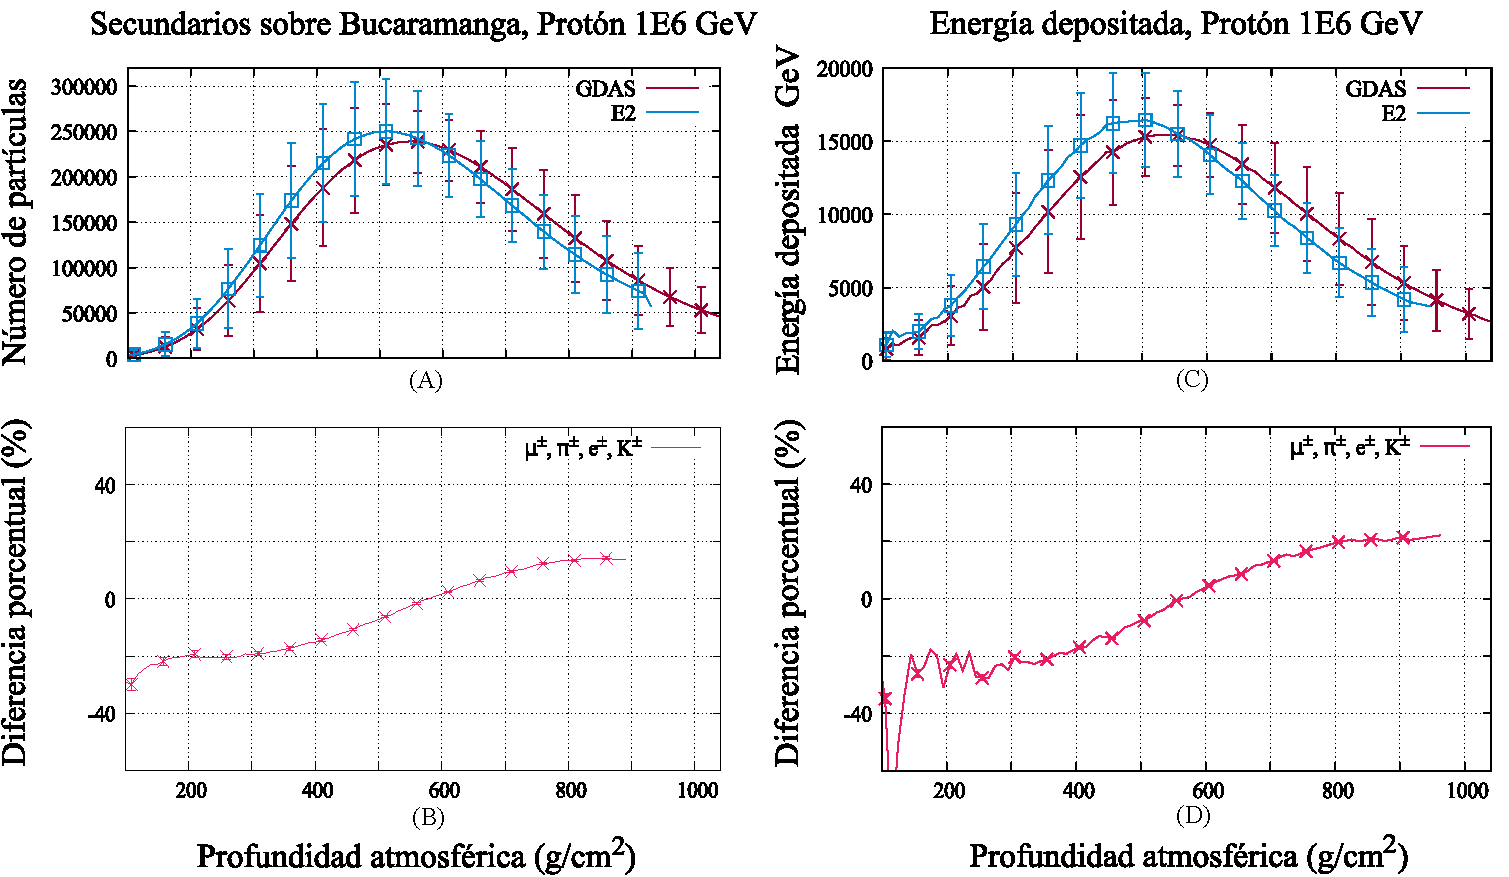
\includegraphics[width=1\textwidth]{Figs/proton_1E6.pdf}
\caption[Distribución longitudinal de un protón de $1\cdot 10^{6} GeV$.]{Distribución longitudinal de un protón de $1\cdot 10^{6} GeV$ que fue simulado 1000 veces, usando la atmósfera predeterminada (línea azul), y usando la atmósfera construida para el mes de abril (línea roja). Se observa el número de partículas que se genera, a medida que la EAS se desarrolla a través de la atmósfera (A), la diferencia porcentual en relación al número de partículas generadas con la atmósfera predeterminada (B), la energía depositada a lo largo del desarrollo de la EAS (C), y la diferencia porcentual en relación a la energía depositada con la atmósfera predeterminada (D).}
\label{fig:fig23}
\end{figure}

Se puede observar, un exceso en el número de partículas generadas longitudinalmente, en la región cercana al $X_{max}$ usando el perfil predeterminado por CORSIKA. Sin embargo, la integral de la gráfica de energía depositada, tiene un 99$\%$ de coincidencia.\\
%Lo anterior sugiere que aunque la atmósfera sea distinta, la energía total que deposita el primario es independiente del medio de interacción.\\

Adicionalmente, la figura \ref{fig:fig24} y la \ref{fig:fig25} muestran los resultados obtenidos para el fotón y un núcleo de hierro, donde pequeñas diferencias cerca del $X_{max}$ también se observan. Las distribuciones longitudinales obtenidas para otros valores de energía se asemejan a lo observado en las figuras \ref{fig:fig23}, \ref{fig:fig24} y \ref{fig:fig25} y se encuentran en el apéndice B.\\

\begin{figure}[htb!]
\centering
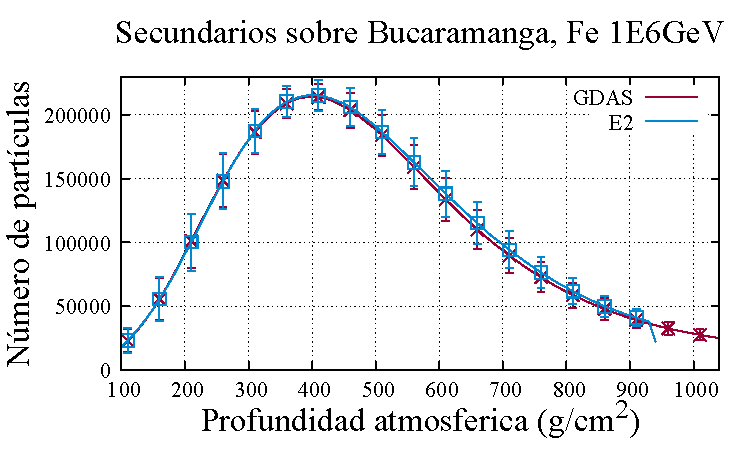
\includegraphics[width=0.6\textwidth]{Figs/longi_fe_1E6_E2_GDAS.pdf}
\caption[Distribución longitudinal de un fotón de $1\cdot 10^{6} GeV$.]{Distribución longitudinal de un fotón de $1\cdot 10^{6} GeV$ que fue simulado 1000 veces, usando la atmósfera predeterminada (línea azul), y usando la atmósfera construida para el mes de abril (línea roja), se observa el número de partículas que se genera, a medida que la EAS se desarrolla a través de la atmósfera.}
\label{fig:fig24}
\end{figure}

\begin{figure}[htb!]
\centering
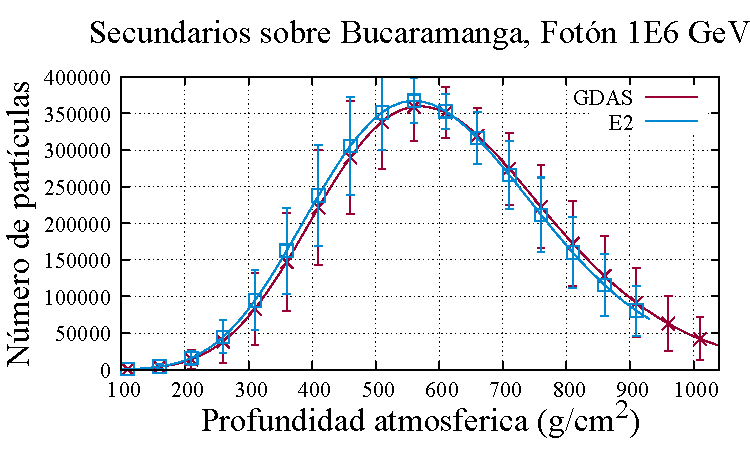
\includegraphics[width=0.6\textwidth]{Figs/longi_foton_1E6_E2_GDAS.pdf}
\caption[Distribución longitudinal de un átomo de hierro de $1\cdot 10^{6} GeV$.]{Distribución longitudinal de un átomo de hierro de $1\cdot 10^{6} GeV$ que fue simulado 1000 veces, usando la atmósfera predeterminada (línea azul), y usando la atmósfera construida para el mes de abril (línea roja), se observa el número de partículas que se genera, a medida que la EAS se desarrolla a través de la atmósfera.}
\label{fig:fig25}
\end{figure}

En particular, la tabla 3 muestra las diferencias porcentuales entre los $X_{max}$ de cada una de las simulaciones realizadas. Las diferencias encontradas no superan el 10$\%$. Esto muestra que la variación en los perfiles atmosféricos afecta el número de partículas generadas cerca al $X_{max}$, e incluso, puede afectar en el flujo, pero la posición del  $X_{max}$ no se ve alterada enormemente.

%teniendo en cuenta que los observatorios de astropartículas tienen una resolución de 26 $g/cm^{2}$  \citepp{Xmax}, es un resultado que concuerda con la idea de que el valor del $X_{max}$ puede ser utilizado para calcular la masa del primario inicial, independientemente del medio de interacción.\\

\begin{table}[]
\small
\begin{minipage}{1\textwidth}
			\caption[Xmax para protones, hierros y fotones de 1E3, 1E6 y 1E8 GeV con y sin GDAS.]{ \raggedright Xmax para protones, hierros y fotones de 1E3, 1E6 y 1E8 GeV con y sin GDAS. La última columna muestra las diferencias porcentuales entre los $X_{max}$ de cada una de las simulaciones realizadas. Las diferencias encontradas no superan el 10$\%$. }
\end{minipage}
\label{tab:tabla3}
\begin{center}
    
\begin{tabular}{llccc}
\hline
\textbf{Energía (GeV)} & \textbf{Partícula} & \multicolumn{1}{l}{\textbf{Xmax GDAS $(g/cm^{2})$}} & \multicolumn{1}{l}{\textbf{Xmax SubTropical $(g/cm^{2})$}} & \multicolumn{1}{l}{\textbf{Diferencia $\%$}} \\ \hline
 & Protón & 310 & 310 & 0 \\ \cline{2-5} 
\multirow{-2}{*}{\textbf{1E3}} & Fotón & 310 & 310 & 0 \\ \hline
\rowcolor[HTML]{EFEFEF} 
\cellcolor[HTML]{EFEFEF} & Protón & 550 & 510 & 7.84 \\ \cline{2-5} 
\rowcolor[HTML]{EFEFEF} 
\cellcolor[HTML]{EFEFEF} & Hierro & 400 & 400 & 0 \\ \cline{2-5} 
\rowcolor[HTML]{EFEFEF} 
\multirow{-3}{*}{\cellcolor[HTML]{EFEFEF}\textbf{1E6}} & Fotón & 570 & 560 & 1.79 \\ \hline
\rowcolor[HTML]{E3E0E0} 
\cellcolor[HTML]{E3E0E0} & Protón & 620 & 650 & 4.6 \\ \cline{2-5} 
\rowcolor[HTML]{E3E0E0} 
\cellcolor[HTML]{E3E0E0} & Hierro & 550 & 560 & 1.79 \\ \cline{2-5} 
\rowcolor[HTML]{E3E0E0} 
\multirow{-3}{*}{\cellcolor[HTML]{E3E0E0}\textbf{1E8}} & Fotón & 750 & 720 & 4.16 \\ \hline
\end{tabular}
\end{center}{}
\end{table}


%De la simulación representada en la figura \label{fig:fig19}, se obtiene una diferencia en el flujo total entre 10,22$\%$ y el 24,12$\%$ correspondientes a los meses de noviembre y abril respectivamente. De forma similar, para los muones estas diferencias están entre 9,58$\%$ y 22,25$\%$. Este resultado responde finalmente a la interrogante planteada en el capítulo anterior. Además, permite conclu

